\section{Versuchsaufbau und Durchführung}
\begin{figure}[H]
\centering
  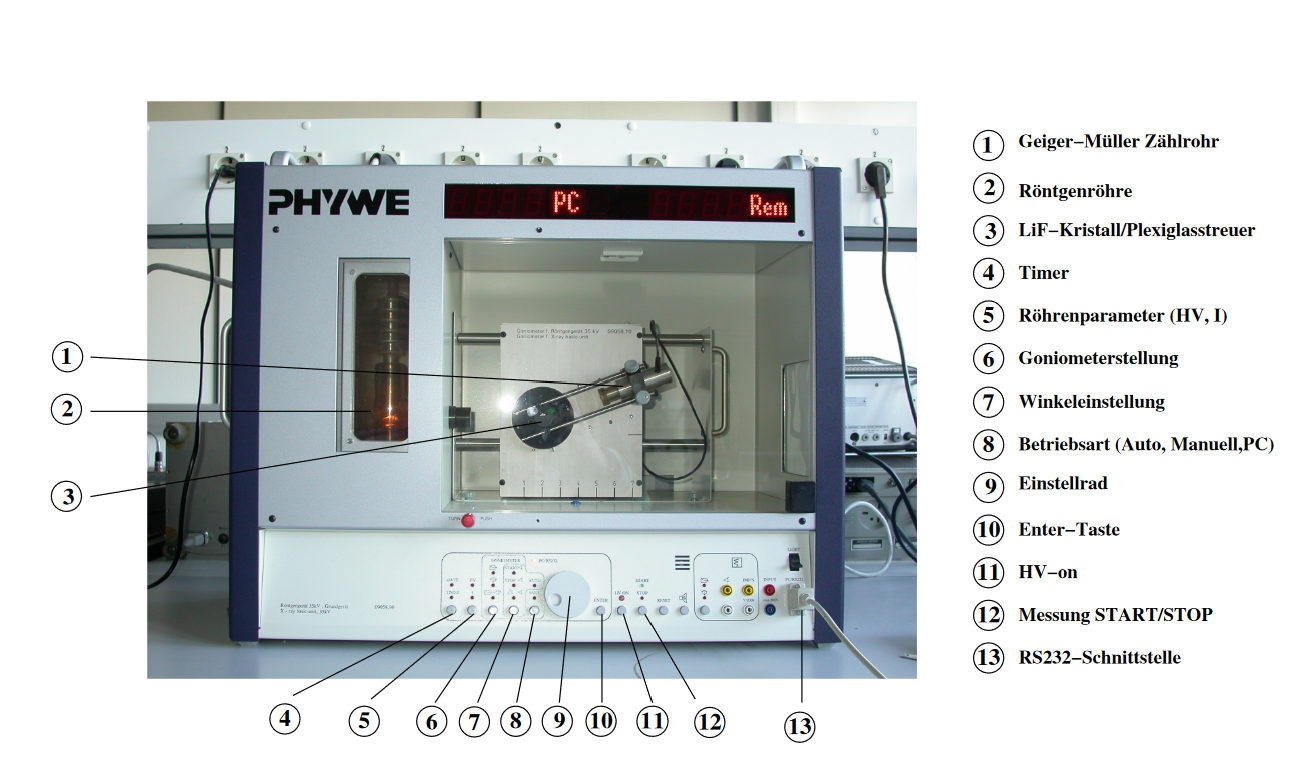
\includegraphics[width=9cm]{content/1.png}
  \caption{Das Messgerät}
  \label{fig:1}
\end{figure}
Für das Experiment wird lediglich eine Kuper-Röntgenröhre, ein KBr-Kristall und ein Geiger-Müller-Zählrohr benötigt. Das alles ist in dem Gerät aus \autoref{fig:1} geschaltet und kann über einen Rechner gesteuert werden. Das Gerät funktioniert mit dem Drehkristallverfahren, bei dem die Wellenlänge gleich bleibt, aber die Bragg-Bedingung für unterschiedliche $\theta$ erfüllt wird. Die Beschleunigungsspannung wird auf $U=35\ \si{\keV}$ und der Emissionsstrom auf $I=1\ \si{\mA}$ gestellt.

\subsection{Überprüfung der Bragg-Bedingung}
Der KBr-Kristall wird auf einen festen Winkel von $\theta=14^{\circ}$ gestellt. Dann soll das Geiger-Müller-Zählrohr den Winkelbereich zwischen $\alpha_{1}=26^{\circ}$ und $\alpha_{2}=30^{\circ}$ in $\Delta\alpha=0.1^{\circ}$-Schritten mit einer Integrationszeit von $\Delta t=5\ \si{\s}$ pro Winkel die Intensität messen.

\subsection{Emissionsspektrum einer Cu-Röntgenröhre}
Zum Messen des Emissionsspektrums einer Cu-Röntgenröhre wir das Programm auf den 2:1 Koppelmodus gestellt und dann das Röntgenspektrum der Beugungsordnung $n=1$ im Winkelbereich zwischen $4^{\circ}\leq\theta\leq 26^{\circ}$ in $\Delta\alpha=0.2^{\circ}$-Schritten mit Integrationszeit $\Delta t=5\ \si{\s}$ gemessen. Der Koppelmodus 2:1 sagt aus, dass während der Kristall um $0.1$° gedreht, das Geiger-Müller-Zählrohr um $0.2$° gedreht wird. Das muss passieren, um die Bragg-Bedingung zu erfüllen. 

\subsection{Absorptionsspektrum}
Es sollen fünf Absorber mit Kernladungszahlen $30\leq Z\leq 50$ vor das Geiger-Müller-Zählrohr gesetzt werden und das Absorptionsspektrum in $\Delta\alpha=0.1^{\circ}$-Schritten mit Integrationszeit $\Delta t=20\ \si{\s}$ gemessen werden. Der Winkelbereich ist variabel.

\section{Vorbereitung}
Zur Vorbereitung sollte ermittelt werden, bei welchen Energien in keV die $\textrm{Cu}-K_{\alpha}$- und $\textrm{Cu}-K_{\beta}$-Linie zu erwarten ist. Diese liegen bei $E_{\textrm{Cu}-K_{\alpha}}=8.05 \si{\keV}$ und $E_{\textrm{Cu}-K_{\beta}}=8.91 \si{\keV}$. Die Glanzwinkel errechnen sich unter der Benutzung von \eqref{1} und \eqref{7} zu $\theta_{\alpha}=13.5^\circ$ und $\theta_{\beta}=12.2^\circ$.
Zusätzlich dazu sollte von Zn, Ge, Br, Rb, Sr und Zr die Absorptionskanten $E_{K}$, der Glanzwinkel $\theta_{K}$ und die Abschirmkonstante $\sigma_{K}$ gefunden werden:
\begin{table}[H]
  \centering
  \begin{tabular}{l|l|l|l|l}
  & Z & $E_{K}$ [keV] & $\theta_{K}$ [$^{\circ}$] & $\sigma_{K}$ \\\hline
  Zn & $30$ & $9.65$ & $11.3$ & $3.56$\\\hline
  Ga & $31$ & $10.37$ & $10.5$ & $3.61$\\\hline
  Ge & $32$ & $11.10$ & $9.8$ & $3.68$\\\hline
  Br & $35$ & $13.47$ & $8.0$ & $3.85$\\\hline
  Rb & $37$ & $15.80$ & $7.1$ & $3.94$\\\hline
  Sr & $38$ & $16.10$ & $6.7$ & $3.99$\\\hline
  Zr & $40$ & $18.00$ & $6.0$ & $4.09$\\\hline
  \end{tabular}
  \caption{Stoffe und deren theoretische Ordnungszahlen, Absorptionskanten, Glanzwinkel und Abschirmkonstanten.}
  \label{tab:1}
\end{table}
